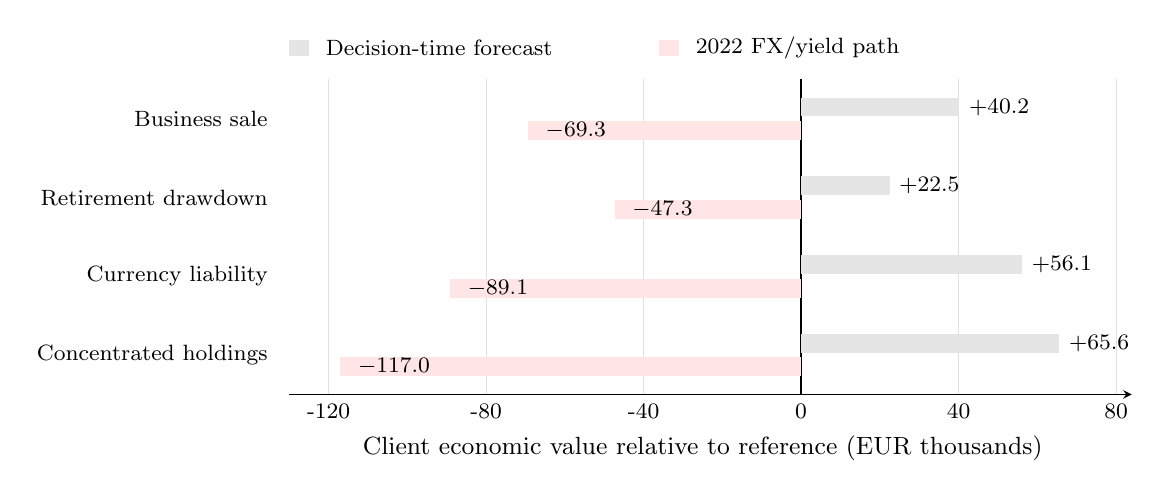
\begin{tikzpicture}[font=\small,>=stealth]
  \draw[gray!25] (0.500,0.35) -- (0.500,4.35);
  \node[below,font=\footnotesize] at (0.500,0.35) {-120};
  \draw[gray!25] (2.500,0.35) -- (2.500,4.35);
  \node[below,font=\footnotesize] at (2.500,0.35) {-80};
  \draw[gray!25] (4.500,0.35) -- (4.500,4.35);
  \node[below,font=\footnotesize] at (4.500,0.35) {-40};
  \draw[gray!25] (6.500,0.35) -- (6.500,4.35);
  \node[below,font=\footnotesize] at (6.500,0.35) {0};
  \draw[gray!25] (8.500,0.35) -- (8.500,4.35);
  \node[below,font=\footnotesize] at (8.500,0.35) {40};
  \draw[gray!25] (10.500,0.35) -- (10.500,4.35);
  \node[below,font=\footnotesize] at (10.500,0.35) {80};
  \draw[thick] (6.5,0.35) -- (6.5,4.35);
  \draw[->] (0,0.35) -- (10.7,0.35);
  \node[left,align=right,font=\footnotesize] at (-.15,3.85) {Business sale};
  \fill[fill=gray!20] (6.50000,3.88) rectangle (8.50821,4.12);
  \node[right,font=\footnotesize] at (8.50821,4.00) {$+40.2$};
  \fill[fill=red!10] (3.03275,3.58) rectangle (6.50000,3.82);
  \node[anchor=west,text=black,font=\footnotesize] at (3.13275,3.70) {$ -69.3 $};
  \node[left,align=right,font=\footnotesize] at (-.15,2.85) {Retirement drawdown};
  \fill[fill=gray!20] (6.50000,2.88) rectangle (7.62358,3.12);
  \node[right,font=\footnotesize] at (7.62358,3.00) {$+22.5$};
  \fill[fill=red!10] (4.13346,2.58) rectangle (6.50000,2.82);
  \node[anchor=west,text=black,font=\footnotesize] at (4.23346,2.70) {$ -47.3 $};
  \node[left,align=right,font=\footnotesize] at (-.15,1.85) {Currency liability};
  \fill[fill=gray!20] (6.50000,1.88) rectangle (9.30515,2.12);
  \node[right,font=\footnotesize] at (9.30515,2.00) {$+56.1$};
  \fill[fill=red!10] (2.04415,1.58) rectangle (6.50000,1.82);
  \node[anchor=west,text=black,font=\footnotesize] at (2.14415,1.70) {$ -89.1 $};
  \node[left,align=right,font=\footnotesize] at (-.15,0.85) {Concentrated holdings};
  \fill[fill=gray!20] (6.50000,0.88) rectangle (9.77818,1.12);
  \node[right,font=\footnotesize] at (9.77818,1.00) {$+65.6$};
  \fill[fill=red!10] (0.64962,0.58) rectangle (6.50000,0.82);
  \node[anchor=west,text=black,font=\footnotesize] at (0.74962,0.70) {$ -117.0 $};
  \fill[fill=gray!20] (0,4.65) rectangle (.25,4.85);
  \node[anchor=west,font=\footnotesize] at (.34,4.75) {Decision-time forecast};
  \fill[fill=red!10] (4.7,4.65) rectangle (4.95,4.85);
  \node[anchor=west,font=\footnotesize] at (5.04,4.75) {2022 FX/yield path};
  \node[below] at (5.25,-.05) {Client economic value relative to reference (EUR thousands)};
\end{tikzpicture}
